\documentclass[11pt,a4paper]{article}
\usepackage[margin=2cm]{geometry}
\usepackage[T1]{fontenc}
\usepackage{lmodern}
\usepackage{graphicx}
\usepackage{xcolor}
\usepackage{enumitem}
\usepackage{caption}
\usepackage[compact]{titlesec}
\usepackage[hidelinks]{hyperref}
\setlist{nosep,leftmargin=*}
\captionsetup{font=small}
\setlength{\parskip}{0.4em}
\setlength{\parindent}{0pt}
\emergencystretch=3em
\newcommand{\todo}[1]{\textcolor{red}{[TODO: #1]}}
\newcommand{\code}[1]{\texttt{#1}}

\title{\vspace{-1.5cm}Automated Post-Trade Reconciliation \& Exception Analytics Engine}
\author{Sara Patano, Alberto Tonni, Mehrdad Vafaee\\\small Data-Intensive Computing\\\small Code: \url{https://github.com/mehrdad-vafaee/trade-reconciliation-engine}}
\date{}

\begin{document}
\maketitle
\vspace{-1.2cm}

\section{Overview}
In post-trade processing, the two counterparties of a transaction each keep their own record of it, and small differences between those records, known as \emph{trade breaks}, have to be found and resolved before settlement.
In this project we built an automated engine that reconciles two such feeds and analyses the exceptions it finds.
Starting from a public dataset of card transactions, we simulate two broker feeds, one clean and one with injected errors.
The engine matches them record by record and labels each discrepancy by type.
Records that cannot be compared are kept in a separate quarantine table together with the reason they were rejected.
The pipeline runs on Apache Spark and is orchestrated by Apache Airflow.
The results are loaded into Google BigQuery and explored in a Looker Studio dashboard.

\section{Dataset}
The pipeline starts from the \emph{Financial Transactions Dataset: Analytics} available on Kaggle\footnote{\url{https://www.kaggle.com/datasets/computingvictor/transactions-fraud-datasets}}.
We use its \code{transactions\_data.csv} file, which contains 13,305,915 card transactions with 12 attributes, and keep the six needed for matching and data-quality checks: \code{id}, \code{date}, \code{client\_id}, \code{card\_id}, \code{amount} and \code{merchant\_id}.
The \code{id} uniquely identifies a transaction, while the other fields record when it happened, the client and card involved, the amount and the merchant.

\section{Data Preparation}
Real bilateral feeds are not publicly available, so we simulate them from this dataset.
Feed A keeps the records unchanged and is the reference.
Feed B starts as a copy of A, and about 75\% of its rows receive exactly one error, chosen at random among 20 types:
\begin{itemize}
  \item realistic changes that should be reported as breaks: a shifted timestamp, or a different amount, client, card or merchant;
  \item small differences within tolerance (under a minute on the date, 0.01 on the amount), which should still count as matched;
  \item invalid values: missing (about 2\% of rows), unparseable or outside the valid range;
  \item a changed transaction id (about 0.5\% of rows), which leaves the record without a counterpart.
\end{itemize}
The generator draws a new seed and new weights for the error types on every run, so each run exercises a different mix of errors.
The seed is saved together with the number of rows that should end up in each outcome, so any run can be reproduced, and the reconciliation step uses these counts to check its own results.

\section{Methodology}
Figure~\ref{fig:arch} shows the architecture of our pipeline, which runs locally with Docker Compose and sends its results to the cloud.

\begin{figure}[h]
  \centering
  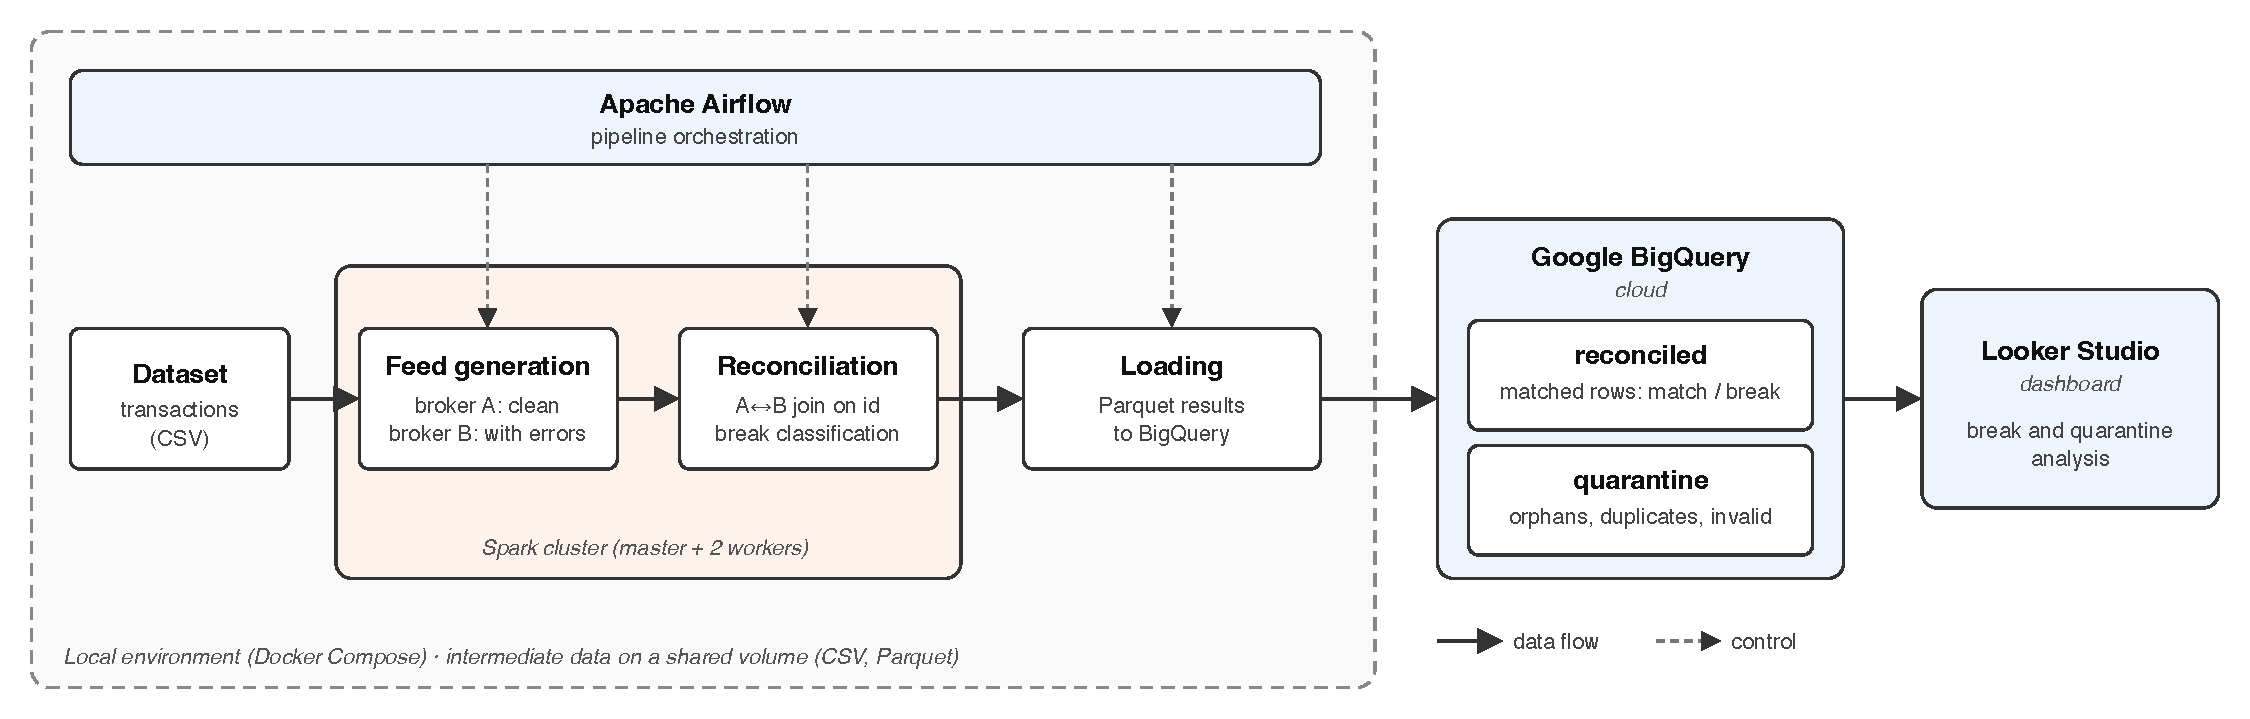
\includegraphics[width=\textwidth]{architecture.pdf}
  \caption{Pipeline architecture.}
  \label{fig:arch}
\end{figure}

\begin{itemize}
  \item \textbf{Apache Airflow} orchestrates the pipeline, starting each step only after the previous one has finished.
  \item \textbf{Feed generation} reads the source dataset and creates the two broker feeds: A as the clean reference, B with injected errors.
  \item \textbf{Reconciliation} validates every field and joins the two feeds on the transaction id. Each pair is labelled as matched or as a break on the field that differs, allowing up to 60 seconds on the date and 0.01 on the amount. Rows with invalid values, a duplicated id or no counterpart go to quarantine with the reason and the column that caused it.
  \item \textbf{Spark cluster} runs the two steps above, splitting the work between one master and two workers (2 cores and 2\,GB each).
  \item \textbf{Loading} uploads the results to Google BigQuery.
  \item \textbf{Google BigQuery} stores them in two tables: \code{reconciled} for matched and broken pairs, \code{quarantine} for the rows set aside. Four SQL views (\code{bigquery/views.sql}) compute on top of them the exposure of each trade and the per-client and per-break-type aggregates used by the dashboard.
  \item \textbf{Looker Studio} reads the two tables and presents the breaks and quarantined rows in a dashboard.
\end{itemize}

\subsection{Distributed implementation}
Both feeds are read as plain strings and converted with Spark's \code{try\_cast} functions, which return null instead of failing on a bad value; this lets a single pass tell missing values (\code{NULL\_VALUE}) from malformed ones (\code{UNPARSEABLE}) and from values outside the valid range (\code{OUT\_OF\_DOMAIN}).
Duplicate ids are detected with a window function, \code{count(*)} over a window partitioned by \code{id}, so no separate aggregation and self-join is needed.
Rows whose id is unusable are removed before the join, and the remaining rows of A and B are combined with a \code{FULL OUTER JOIN} on \code{id}: a missing side becomes \code{MISSING\_IN\_A} or \code{MISSING\_IN\_B}.
Spark executes the join as a shuffle on the join key, so rows with the same id end up in the same partition and the work is spread across both workers.
The break checks are plain column expressions evaluated in the same stage, without user-defined functions, so Spark can optimise the whole plan.
Because the joined result feeds two outputs (reconciled and quarantine), it is persisted to disk once instead of being recomputed; we use \code{DISK\_ONLY} storage to stay within the 2\,GB of memory of each worker.
Each output is written as a single Parquet file, which BigQuery loads in one job.
In BigQuery, \code{reconciled} is partitioned by month and clustered by \code{status}, and \code{quarantine} is clustered by \code{reason}, so the dashboard queries scan only the blocks they need.

\section{Results}
For every run, the reconciliation job compares the number of rows in each status and quarantine reason with the counts recorded by the generator, and fails if any of them differs.
Since a failed check stops the DAG before the loading step, every run that reaches the dashboard has passed it.
On our local machine, the whole pipeline on the 13.3 million rows takes about 12 minutes, from starting the containers to the updated dashboard.

The results are presented in a Looker Studio dashboard (Figure~\ref{fig:dash}).
The top row shows the main KPIs: total reconciled pairs, matched pairs, breaks and total exposure, defined as the sum over all pairs of the absolute difference between the amounts reported by A and B.
Below, the dashboard shows the ten clients with the highest exposure, the distribution of break types, and a table of the quarantined rows with the reason and the column that caused them.

\begin{figure}[h]
  \centering
  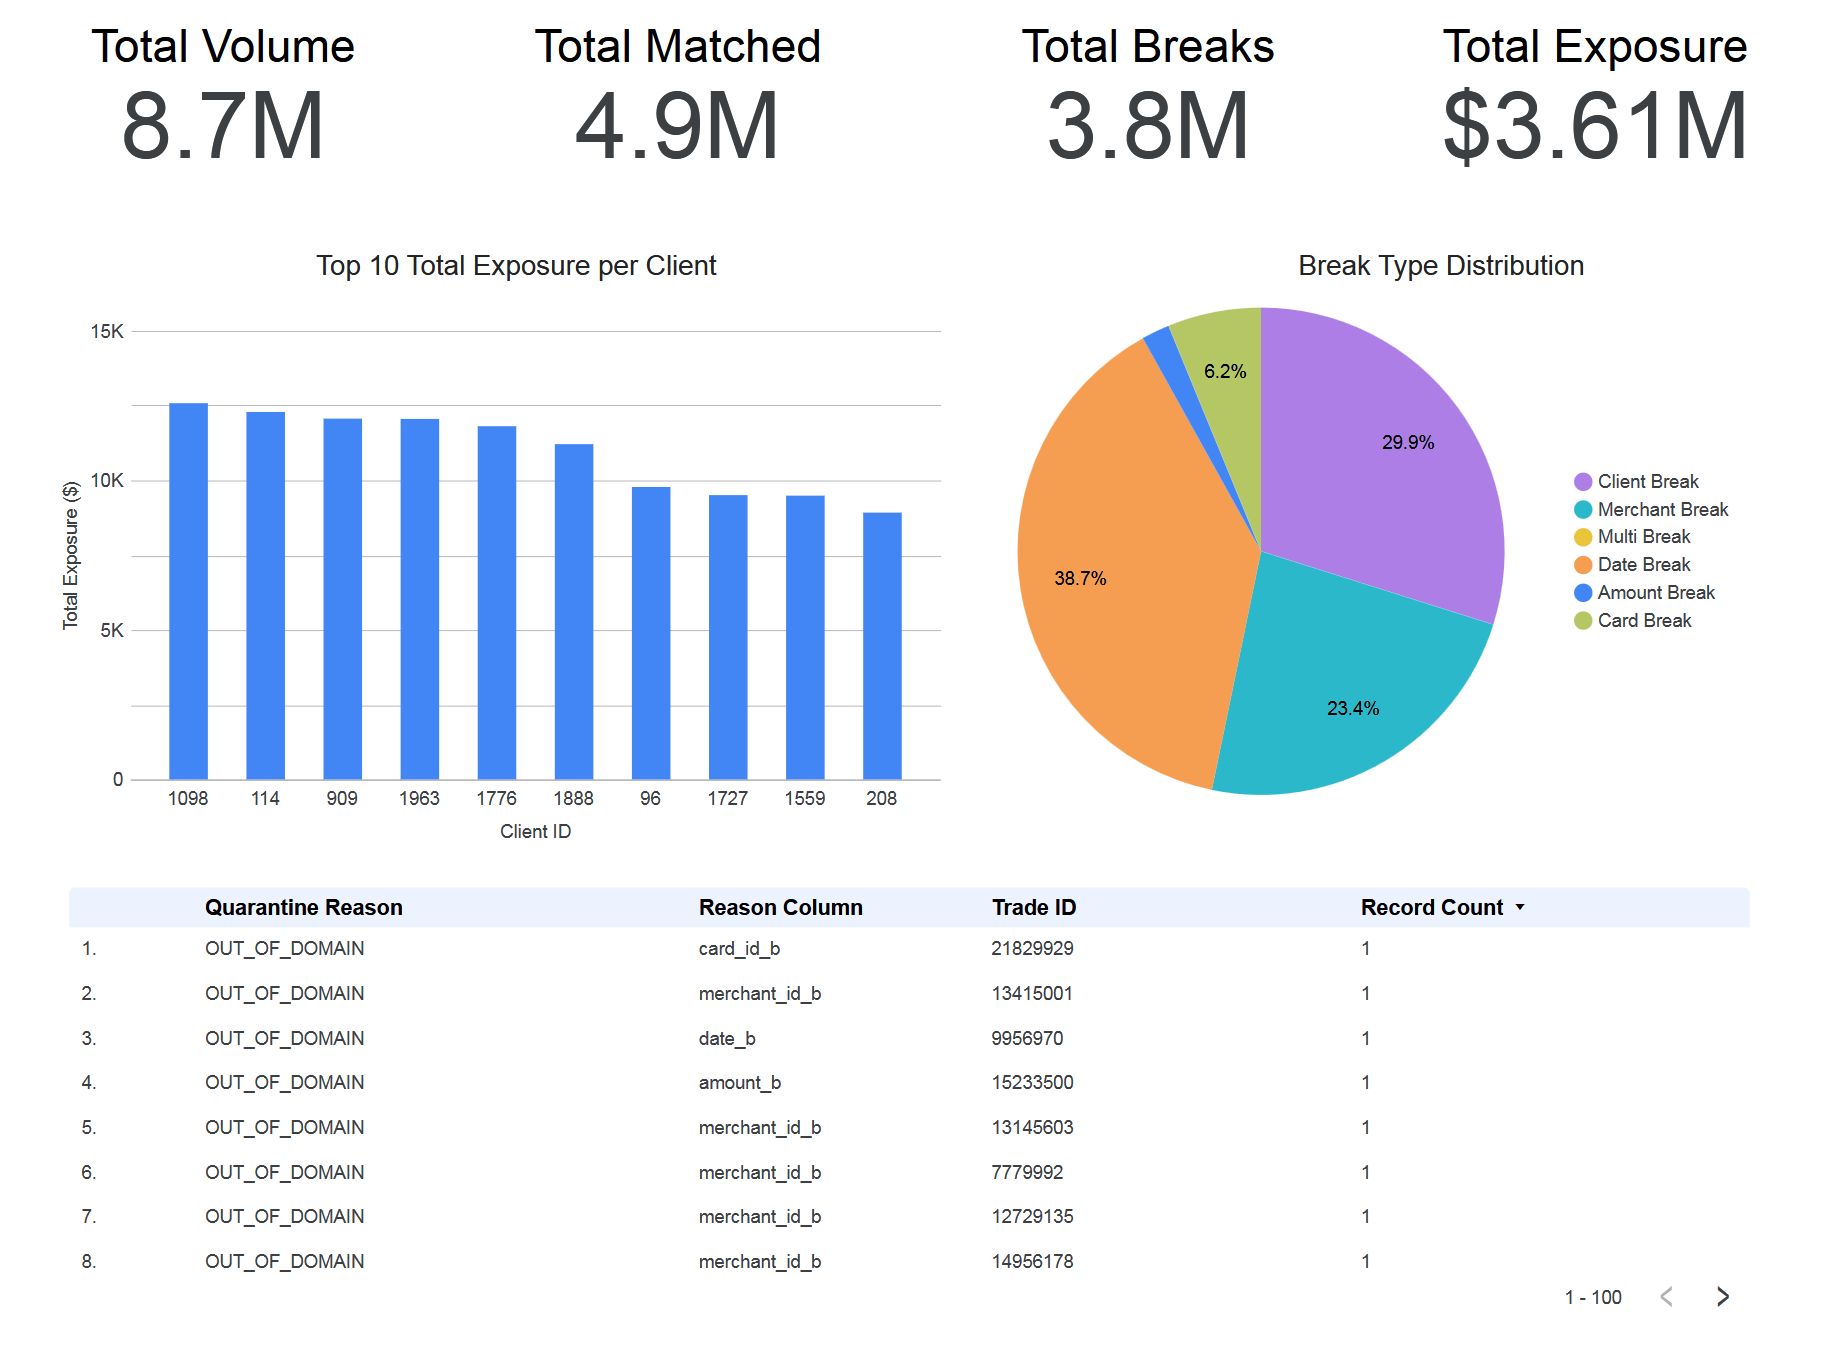
\includegraphics[width=0.7\textwidth]{dashboard.png}
  \caption{Dashboard produced in Looker Studio.}
  \label{fig:dash}
\end{figure}

\section{Limitations and Future Work}
The feeds are simulated, and every row of B carries at most one error, so the \code{MULTI\_BREAK} status is never produced; real feeds would also need fuzzy matching when ids differ.
Intermediate data lives on a shared Docker volume rather than on HDFS, which is enough for a single machine but would be replaced by HDFS or Cloud Storage on a real cluster.
The pipeline runs as a batch on demand; the next step is a daily schedule fed by market data APIs, and moving the BigQuery views into dbt models with automated data tests.

\section{Running the Code}
\textbf{Requirements:} Docker, and a Google Cloud project with BigQuery and a service account key.

\textbf{Setup}
\begin{enumerate}
  \item Save the Kaggle file \code{transactions\_data.csv} as\\\code{data/source/transactions\_data-selected-columns.csv}.
  \item Place the service account key in \code{secrets/gcp-key.json}.
  \item In the BigQuery console, run \code{bigquery/schema.sql} to create the tables, then \code{bigquery/views.sql} to create the views.
\end{enumerate}

\textbf{Run}
\begin{enumerate}[resume]
  \item Start the containers with \code{docker compose up --build}.
  \item Open Airflow at \code{localhost:8081} and trigger the \code{trade\_reconciliation} DAG. Spark progress is visible at \code{localhost:8080}.
  \item Results appear in BigQuery under \code{trade\_reconciliation\_dev}, in the \code{reconciled} and \code{quarantine} tables.
\end{enumerate}

\end{document}
